\documentclass[]{AVSSimReportMemo}
\usepackage{AVS}

\newcommand{\ModuleName}{orbitAxisSpin}
\newcommand{\subject}{Guidance Module to Perform a Constant Spinning about an Orbit Axis}
\newcommand{\status}{Initial Version}
\newcommand{\preparer}{M. Cols}
\newcommand{\summary}{Generate the attitude reference to achieve a spinning motion about a primary orbit frame axis. A chosen reference axis $\hat{r}_{j} = \hat{r}_{spin}$ is to line up with the orbit axis $\hat{o}_{i} = \hat{o}_{spin}$, and rotate a desired rate $\omega_{spin}$}


\begin{document}

\makeCover


%
%	enter the revision documentation here
%	to add more lines, copy the table entry and the \hline, and paste after the current entry.
%
\pagestyle{empty}
{\renewcommand{\arraystretch}{2}
\noindent
\begin{longtable}{|p{0.5in}|p{4.5in}|p{1.14in}|}
\hline
{\bfseries Rev}: & {\bfseries Change Description} & {\bfseries By} \\
\hline
Draft & initial copy & M. Cols \\
\hline

\end{longtable}
}

\newpage
\setcounter{page}{1}
\pagestyle{fancy}

\tableofcontents
~\\ \hrule ~\\

\begin{figure}[htb]
	\centerline{
	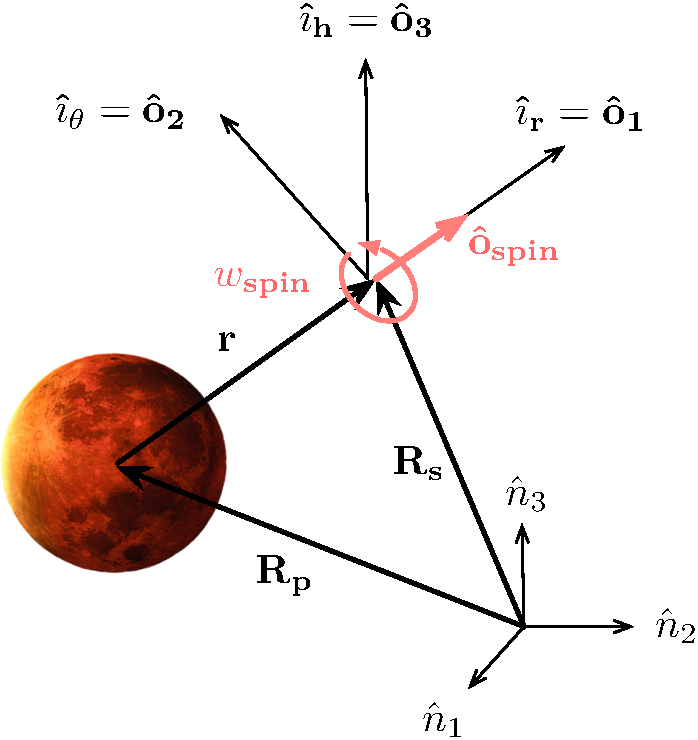
\includegraphics[width=5cm]{Figures/Fig1}
	}
	\caption{Illustration of spinning about the nadir orbit axis $\bm\hat{\imath}_{r}$ of the Hill orbit frame $\mathcal{H}$  at a constant rate $\omega_{\textrm{spin}}$.}
	\label{fig:Fig1}
\end{figure}

\section{Introduction}
In this note a method is discussed on how to compute the reference frame angular rate $\bm\omega_{R/N}$ and acceleration $\dot{\bm\omega}_{R/N}$ to achieve a particular family of stabilized spin motion. This module receives as input the generated reference for a constaint pointing towards an orbit reference frame. Let us call the input reference $\mathcal{R}_{0}$. The goal is now to create a new reference $\mathcal{R}$ that spins about any of the orbit axes, $\hat {o}_{\textrm{spin}}$, at a constant rate $\omega_{\textrm{spin}}$. Note that the presented method is general enough to use any of the Hill $\mathcal{H}:\{ \hat{\bm\imath}_{r}, \hat{\bm\imath}_{\theta}, \hat{\bm\imath}_{h} \}$ or Velocity $\mathcal{V}:\{ \hat{\bm\imath}_{n}, \hat{\bm\imath}_{v}, \hat{\bm\imath}_{h} \}$ orbit frame orientations as the input reference. Figure 1 illustrates the case in which $\mathcal{R}_{0}$ is aligned with $\mathcal{H}$ and the spinning is about the nadir axis $\hat{\bm\imath}_{r}$.

\section{Angular Velocity and Acceleration Descriptions}
The reference frame $\mathcal{R}$ is defined above, and the attitude reference frame tracking control requires the angular rate $\bm\omega_{R/N}$ and acceleration $\dot{\bm\omega}_{R/N}$. 
Let the MRP attitude set, angular velocity vector and angular acceleration vector associated with the constant pointing reference be $\bm\sigma_{
R_{0}/N}$, $\bm\omega_{R_{0}/N}$ and $\bm\dot{\omega}_{R_{0}/N}$ respectively.
The angular velocity of the spinning reference frame is thus given by:
\begin{subequations}
	\label{eq:omegaRN}
	\begin{equation}
		\bm\omega_{R/N} = \bm\omega_{\textrm{spin}} + \bm\omega_{R_{0}/N} 
	\end{equation}
	\begin{equation}
		\bm\omega_{R/N} = {\omega}_{\textrm{spin}}\hat{o}_{\textrm{spin}} + \bm\omega_{R_{0}/N}
	\end{equation}
\end{subequations}
Since $\hat {o}_{\textrm{spin}}$ is aligned with one of the orbit axis defining $\mathcal{R}_{0}$, taking the inertial derivative of ~\eqref{eq:omegaRN}:
\begin{subequations}
	\label{eq:domegaRN}
	\begin{equation}
		\dot{\bm\omega}_{R/N} = \dot{\bm\omega}_{\textrm{spin}} +\dot{\bm\omega}_{R_{0}/N} 
	\end{equation}
	\begin{equation}
		\dot{\bm\omega}_{R/N} = \frac{^{\mathcal{R}_{0}} \textrm{d}}{\textrm{dt}} (\omega_{\textrm{spin}}\bm\hat{o}_{\textrm{spin}}) + \bm\omega_{R_{0}/N}\times (\omega_{\textrm{spin}}\bm\hat{o}_{\textrm{spin}}) + \bm{\dot\omega}_{R_{0}/N}
	\end{equation}
\end{subequations}
\section{MRP Attitude Set}
Let be $\phi_{\textrm{spin}}$ be the current spin angle that the reference frame has rotated about its spin axis $\hat o_{\textrm{spin}}$. The final reference frame orientation is eventually given by
\begin{equation}
	\label{eq:dbeta}
	[RN] =  [M_{\hat{o}_{\textrm{spin}}} (\phi_{\textrm{spin}})][R_{0}N]
\end{equation}
where $[R_{0}N]$ is the Direction Cosine Matrix associated with the orbit axis pointing attitude set, and $M_{\hat{o}_{\textrm{spin}}}$ is the principal axis rotation matrix about $\hat o_{\textrm{spin}}$. Assuming a constant spin rate, the spin angle is propagated using the simple Euler integration scheme
\begin{equation}
	\label{eq:dbeta}
	\phi_{\textrm{spin, n+1}} = \phi_{\textrm{spin, n}} + \omega_{\textrm{spin}}\Delta t
\end{equation}
With $[RN]$ defined, the MRP attitude set $\sigma_{R/N}$ can readily be computed.

\section{Spin Angle Initialization Process}
Any alignment between reference frames, say $\mathcal{B}$ and $\mathcal{R}$, can be achieved through a single rotation about a principal rotation axis. If $\phi_{\textrm{align}}$ is the principal rotation angle, then the alignment can be achieved through a rotation of whether $\phi_{\textrm{align}}$ or $( 2\pi - \phi_{\textrm{align}})$. In order to determine the initial spin angle and assure that the chosen path is always the shortest rotation, the original $\mathcal{B}$ and final $\mathcal{R}$ frame orientations must be known.\par

\subsection{Algorithm Outlines}
The question remains on how to initialize the spin angle $\phi_{\textrm{spin}}$. Since the initialization of the spin angle does not allow further generality in the generatiton of reference attitudes, a separate algorithm is used.
Being $\mathcal{B}$ the body frame and $\mathcal{R}_{0}$ the orbit frame orientations, let us set $\hat{b}_{\textrm{spin}}$ as the principal body axis that is to be aligned with the principal orbit axis $\hat{o}_{\textrm{spin}}$. The triodes of axes $\hat b_{i}$ and $\hat o_{i}$ are labeled so that the first index determines the spin axis, i.e. $\hat b_{1} =\hat b_{\textrm{spin}}$ and $\hat o_{1} =\hat o_{\textrm{spin}}$. The remaining two indices are set to yield a right-handed coordinate frame. Note that $\mathcal{R}_{0}$ could reference to either Hill orbit frame $\mathcal{H}$ or Velocity $\mathcal{V}$.\par

Let $\mathcal{R}$ be the reference orientation in which $\hat o_{1}$ orbit axis and $\hat b_{1}$ body axis are lined up. Using the definition where $RN(i)$ is the $i_{th}$ row of the $[RN]$ DCM matrix:
\begin{equation}
	\label{eq:dbeta}
	RN(\hat b_{1}) = R_{0}N(\hat o_{1}) 
\end{equation}
\begin{equation}
	\label{eq:dbeta}
	RN(\hat b_{2}) = R_{0}N(\hat o_{2}) 
\end{equation}
\begin{equation}
	\label{eq:dbeta}
	RN(\hat b_{3}) = RN(\hat b_{1}) \times RN(\hat b_{2})
\end{equation}
Having $[RN]$ and $[BN]$ defined, the spin axis alignment angle $\phi_{\textrm{align}}$ is computed as the relative orientation between $\hat b_{\textrm{spin}}$ and $\hat o_{\textrm{spin}}$. Next, the body frame is rotated about a principal rotation angle to align these two axes. Eventually, the initial spin angle $\phi_{\textrm{spin}}$ is defined as the smallest angle to align the remaining two.

\bibliographystyle{unsrt}
\bibliography{references}

\end{document}
